\chapter{Descripción de los editores de propósito general}

Nuestro trabajo es repetitivo por naturaleza. Cuando hacemos pequeños cambios en varias partes o moviéndonos alrededor entre regiones similares de un documento, repetimos varias acciones. Cualquier cosas que pueda seguir una línea repetitiva de flujo de trabajo nos ahorrará múltiple tiempo.

Vim está optimizado para la repetición. Su eficiencia proviene de la forma en que rastrea nuestras acciones más recientes. Podemos siempre repetir el último cambio con una sola pulsación de tecla. Por poderoso que parezca, es inútil a menos que aprendamos a diseñar nuestras acciones para que realicen una unidad de trabajo útil cuando se reproducen. Dominar este concepto es la clave para hacerse efectivo con Vim.

El comando punto es nuestro punto de partida. Este comando aparentemente simple es la más versátil herramienta en la caja, y entendiendo este es el primer paso hacia el dominio de Vim. Trabajaremos a través de un puñado de tareas de edición simples que se pueden ejecutar rápidamente completadas con el comando punto. Aunque cada tarea se ve bastante diferente de la siguiente, sus soluciones casi convergen. Identificaremos una fórmula de edición ideal, que requiere solo una pulsación de tecla para moverse y otra para ejecutar.

\begin{figure}[ht!]
\centering
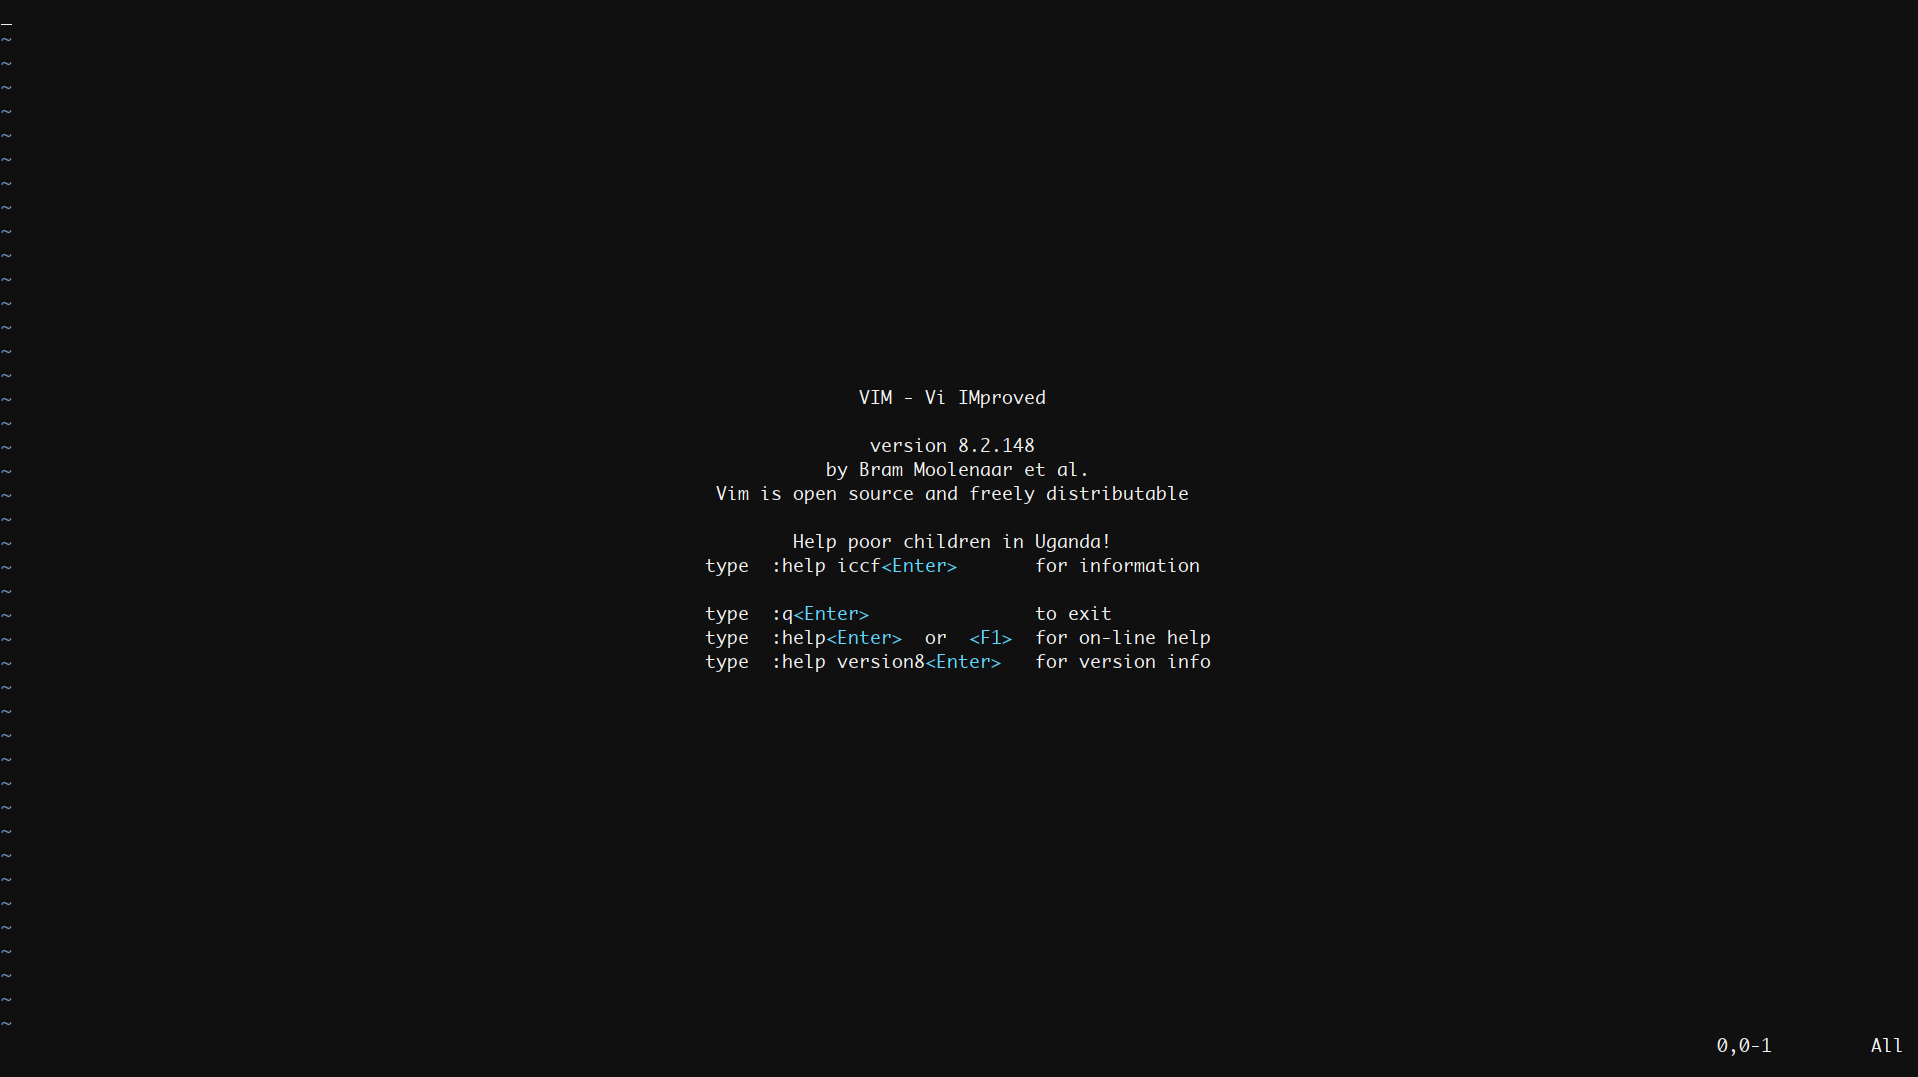
\includegraphics[width=0.8\paperwidth]{./img/VimStart}
\end{figure}

\begin{figure}[ht!]
	\centering
	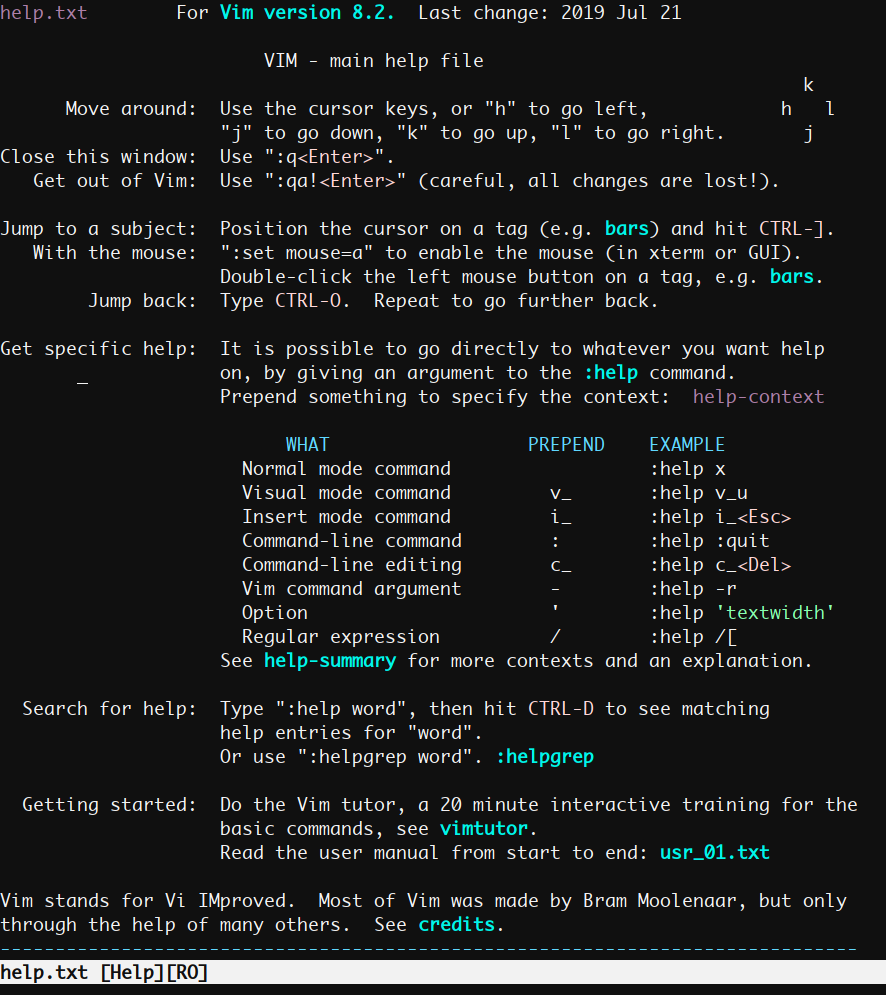
\includegraphics[width=0.8\paperwidth]{./img/VimHelp}
\end{figure}

\section{Vim}
Para entrar al modo de comandos debemos presionar
la tecla \keys{ESC} seguida del símbolo \keys{:}
(dos puntos), y para entrar al modo de edición tenemos que
presionar la tecla \keys{ESC} seguida de alguna de las
siguientes letras:

\mintinline{vim}{a:} entra en modo de edición y agrega el texto
tipeado justro detrás de la posición del cursor.

\mintinline{vim}{i:} entra en modo de edición e inserta el texto
justo delante de la posición actual del cursor.

\mintinline{vim}{A:} Añade el nuevo texto al final de la línea actual
indicada por el cursor.

\mintinline{vim}{I:} inserta el texto al comienzo de la línea indicada
por el cursor.

\mintinline{vim}{O:} inserta una nueva línea entre la línea inferior a la
posición del cursor.

* Para guardar el archivo y continuar editándolo entramos
al modo comando y tipeamos el comando \mintinline{vim}{:w}.

* Para guardar el archivo y salir del editor entramos al
modo comando y tipeamos el comando \mintinline{vim}{:wq}.

* Para salir del editor sin guardar el archivo, entramos al
modo comando y tipeamos el comando \mintinline{vim}{:q!}.

El próximo paso es aprendernos los comandos para desplazarnos
por el contenido de la ventana de Vi. Para todos los siguientes
atajos es necesario presionar antes la tecla ESC para entrar
en modo de comando:

\mintinline{vim}{w:} mover el cursor hacia la siguiente palabra.
\mintinline{vim}{e:} mover el cursor hacia el final de la palabra.
\mintinline{vim}{b:} mover el cursor hacia el comienzo de la palabra.
\mintinline{vim}{):} mover el cursor hacia el inicio de la próxima oración.
\mintinline{vim}{(:} mover el cursor hacia el inicio de la oración actual.
\mintinline{vim}|}:| mover el cursor hacia el inicio del próximo párrafo.
\mintinline{vim}|{:| mover el cursor hacia el inicio del párrafo actual.
\mintinline{vim}{G:} mover el cursor hacia el final del archivo.

También disponemos de algunas combinaciones de teclas para
desplazarnos por la ventana de edición:

\keys{\ctrl+F}: mueve una pantalla completa hacia adelante.
\keys{\ctrl+B}: mueve una pantalla completa hacia atrás.

Ahora vamos a aprender a modificar nuestro texto. El comando
más simple es r, que se encarga de reemplazar el carácter
actual por otro indicado justo a continuación del comando
(como por ejemplo rb). Para borrar caracteres disponemos del
comando x, que acepta prefijos numéricos para definir cuántos
caracteres se deben borrar (por ejemplo 10x). Por su parte. el
comando d es un poco más versátil. Vemos algunas combinaciones:

dw: borra desde la posición
(como por ejemplo)
\keys{\ctrl + F}

\lipsum[1]
\begin{wrapfigure}{r}{0.2\paperwidth}
	\includesvg[width=0.19\paperwidth]{./img/editors/vim}
\end{wrapfigure}
\lipsum[1]

\section{Emacs}

\lipsum[1]
\begin{wrapfigure}{l}{0.2\paperwidth}
	\includesvg[width=0.19\paperwidth]{./img/editors/emacs}
\end{wrapfigure}
\lipsum[1]

\section{Sublime}

\lipsum[1]
\begin{wrapfigure}{r}{0.2\paperwidth}
	\includesvg[width=0.19\paperwidth]{./img/editors/sublime}
\end{wrapfigure}
\lipsum[1]

\section{Visual Studio Code(ium)}

\lipsum[1]
\begin{wrapfigure}{l}{0.2\paperwidth}

\includegraphics[width=0.19\paperwidth]{./img/editors/vscodium}
\end{wrapfigure}
\lipsum[1]

\section{Atom}

\lipsum[1]
\begin{wrapfigure}{r}{0.2\paperwidth}
	
\includegraphics[width=0.19\paperwidth]{./img/editors/atom}
\end{wrapfigure}
\lipsum[1]

`manni' style on a white background:
\usemintedstyle{manni}
\begin{minted}{c}
char *test = "1000";
int *test_int = (int*) test;
printf("Machine is %s-endian", (test_int >> 1)? "big":"little");    
\end{minted}

`vim' style on a dark background:
\usemintedstyle{vim}
% note that minted seems to screw up the placment of the background here
\begin{minted}[bgcolor=black]{c}
char *test = "1000";
int *test_int = (int*) test;
printf("Machine is %s-endian", (test_int >> 1)? "big":"little");  
\end{minted}

Derived `myvim' style on a white background:
\usemintedstyle{myvim}
\begin{minted}{c}
char *test = "1000";
int *test_int = (int*) test;
printf("Machine is %s-endian", (test_int >> 1)? "big":"little");  
\end{minted}